% !TEX root = ../main.tex
\begin{figure}[t]
\vspace{-0.1in}
\centering
\iflatexml
    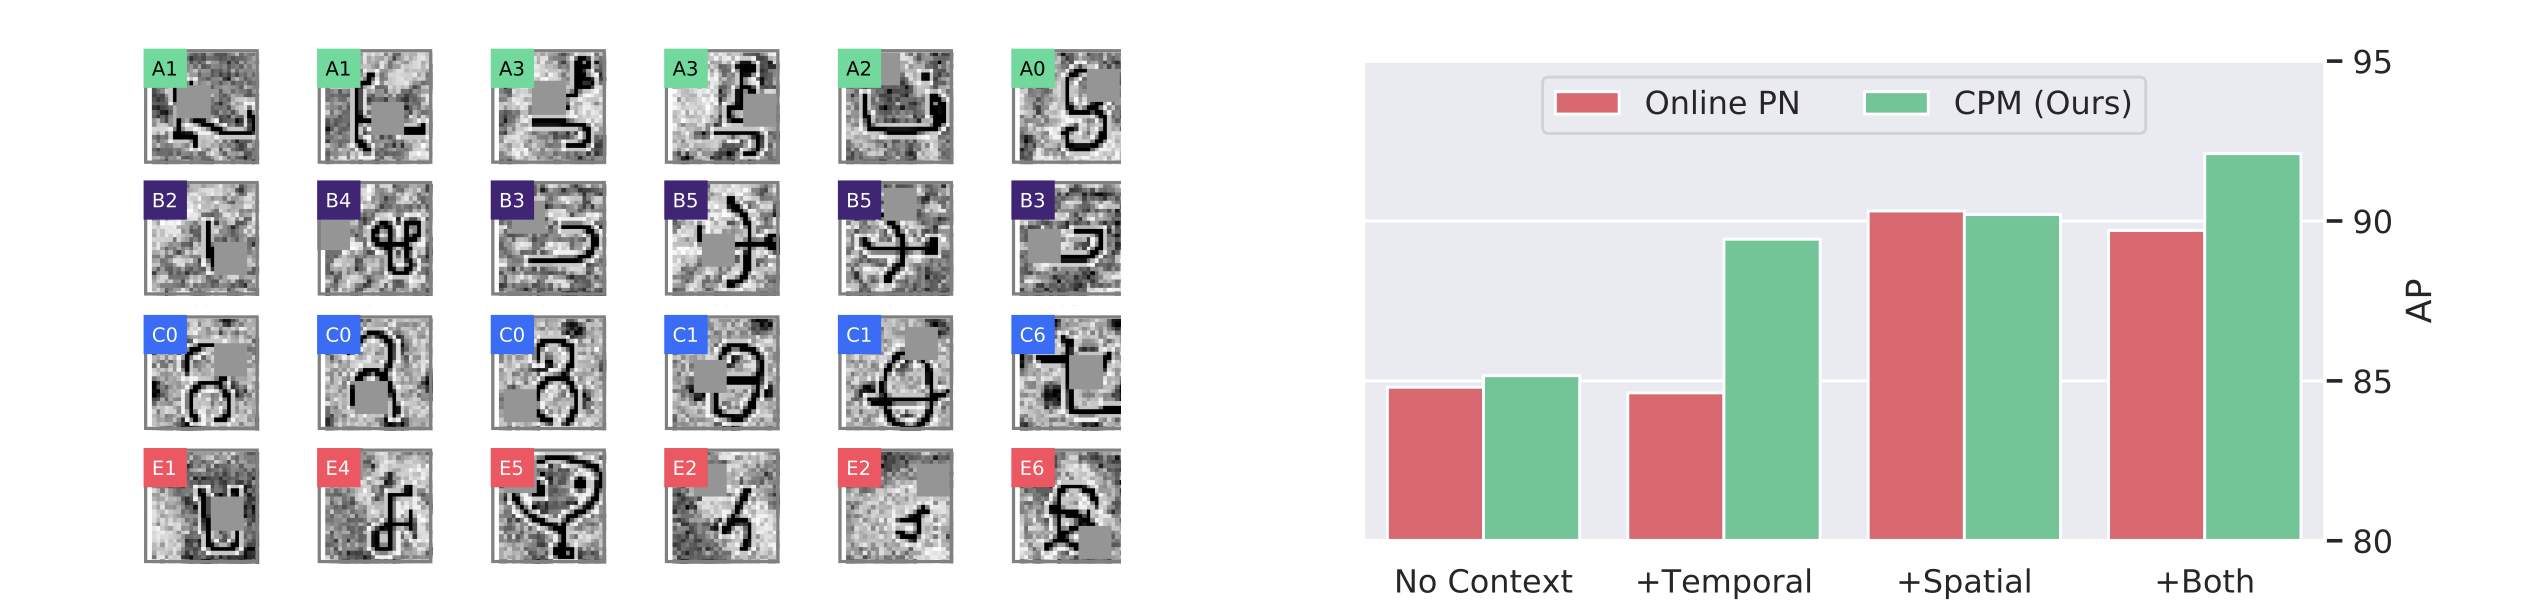
\includegraphics[width=6\linewidth]{figures/spatiotemporal_full.png}
\else
    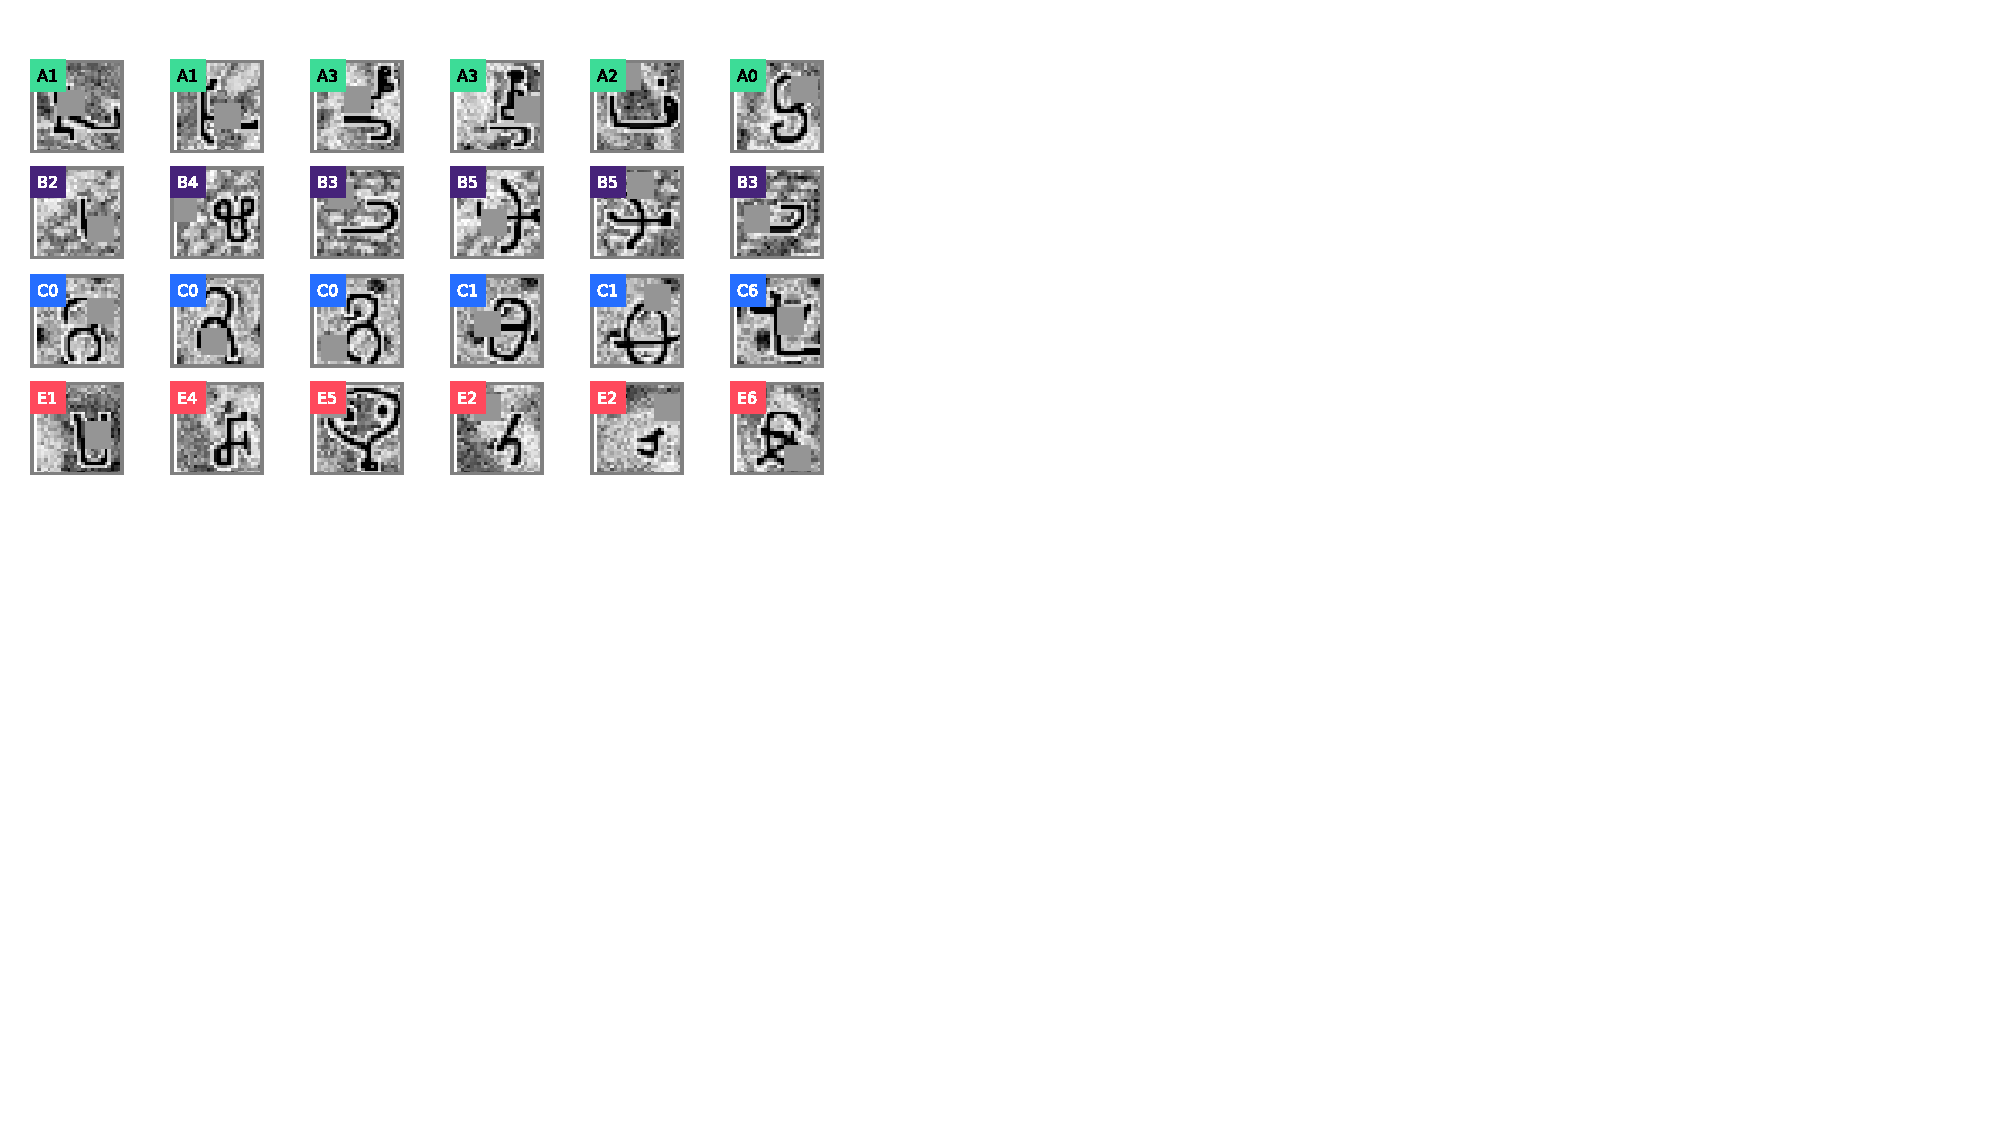
\includegraphics[height=2.8cm,trim={-2.25cm 10cm 20cm 0.5cm},clip]{figures/omniglot-texture.pdf}
    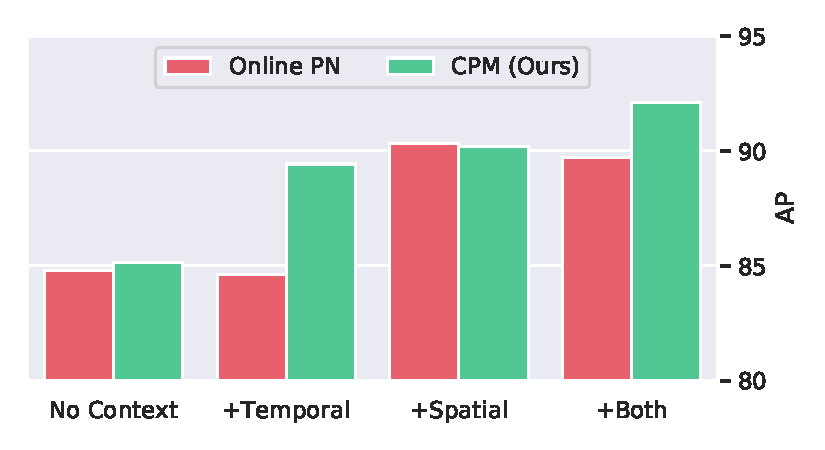
\includegraphics[height=2.8cm,trim={-2.25cm 0 0.5cm 0},clip]{figures/spatiotemporal.pdf}
\fi
\quad
\vspace{-0.2in}
\caption{\textbf{Effect of spatiotemporal context.} Spatiotemporal
context are added separately and together in \ourchar{}, by introducing texture background and
temporal correlation. \textbf{Left:} Stimuli used for spatial cue of the background environment.
\textbf{Right:} Our CPM model benefits from the presence of a temporal context
(``+Temporal'' and ``+Both'')} %, while Spatial context helps both CPM and online ProtoNet.}
\label{fig:spatiotemporal}
% \vspace{-0.1in}
\end{figure}
